
\documentclass[calculator,allquestions,datasheet,solutions]{exam_newMarcus2}
%\documentclass[calculator,allquestions,datasheet,Pens,resit]{exam_newMarcus2}

% The full list of class options are
% calculator : Allows approved calculator use.
% datasheet : Adds a note that data sheet are attached to the exam.
% handbook : Allows the use of the engineering handbook.
% resit : Adds the resit markings to the paper.
% sample : Adds conspicuous SAMPLE markings to the paper
% solutions : Uses the contents of \solution commands (and \solmarks) to generate a solution file

\usepackage{pdfpages}  
\usepackage{lscape,comment} 
 
\coursecode{EX3029}%% 
\coursetitle{Chemical Thermodynamics}
 
\examtime{00.00--00.00}%
\examdate{15}{12}{2017}% 
\examformat{Attempt ALL questions. \\ Each question is worth 20 marks.}

% Other symbols
\newcommand{\frc}{\displaystyle\frac}
\newcommand{\br}[1]{\!\left( #1 \right)}
\newcommand{\abs}[1]{\left| #1 \right|}
\newcommand{\fracd}[2]{\frac{\mathrm{d} #1}{\mathrm{d} #2}}
\newcommand{\fracp}[2]{\frac{\partial #1}{\partial #2}}
\renewcommand{\d}[1]{\mathrm{d} #1 } 
\newcommand{\Ma}{\mathrm{M\!a}} 
\newcommand{\eg}{{\it e.g., }}
\newcommand{\ie}{{\it i.e., }}
\newcommand{\wrt}{{\it wrt }}
\newcommand{\Partial}[3][error]{\left(\frc{\partial #1}{\partial #2}\right)_{#3}}
\newcommand{\mfr}[3][error]{#1_{#2}^{\left(#3\right)}} 
\newcommand{\summation}[3][error]{\sum\limits_{#2}^{#3}#1}


\begin{document}


%%%
%%% Question 01 
%%%
\begin{question}
   An engineering consultancy company is contracted to design a separation process for a mixture of petroleum naphtha and fertilisers by-products. The mixture will be separated by a series of distillation and crystallisation processes. After the first distillation, lighter and heavier streams are stored in two pressure vessels:
         \begin{itemize}
            \item {\bf Vessel 1:} 45 mol$\%$ of n-hexane, 30 mol$\%$ of n-heptane and 25 mol$\%$ of i-octane;
            \item {\bf Vessel 2:} 20 mol$\%$ of n-hexane  and 80 mol$\%$ of chlorobenzene.
         \end{itemize} 
         Vessels 1 and 2 are kept at 1.5 and 1.0 bar, respectively. In order to design the second set of distillations, 
         \begin{enumerate}[a)]
            \item  Estimate the bubble and dew temperatures for Vessel 1. Also calculate the compositions at bubble and dew points;~\marks{8}
                \solution{\begin{enumerate}[i)]
                            \item Bubble point:
                                 \begin{eqnarray}
                                    \sum\limits_{i=1}^{n} y_{i} &=& \sum\limits_{i=1}^{n} \frc{x_{i}P_{i}^{\text{sat}}}{P} = 1 \nonumber \\
                                     &=& \frc{x_{C6}P_{C6}^{\text{sat}}}{P} + \frc{x_{C7}P_{C7}^{\text{sat}}}{P} + \frc{x_{C8}P_{C8}^{\text{sat}}}{P} = 1 \nonumber \\
                                     &=& x_{C6}P_{C6} + x_{C7}P_{C7} + x_{C8}P_{C8} = P, \nonumber 
                                  \end{eqnarray}
                                  with the Antoine relation,
                                  \begin{displaymath}
                                    \ln{P^{\text{sat}}} = A - \frc{B}{T+C},
                                  \end{displaymath}
                                  with $P$ 150 kPa. Solving this non-linear equation (using a calculator) leads to the bubble point temperature $\Longrightarrow$ $T_{\text{bubble}}$ = 95.68$^{\circ}$C~\solmarks{2/8}.  Vapour phase composition is obtained from:
                      \begin{displaymath}
                         y_{i} = \frc{x_{i}P_{i}^{\text{sat}}}{P}.
                      \end{displaymath}
                      Leading to y = [ 0.6603, 0.1870, 0.1527 ]. ~\solmarks{2/8}
%
               \item Dew point:
                    \begin{eqnarray}
                        \sum\limits_{i=1}^{n} x_{i} &=& \sum\limits_{i=1}^{n} \frc{y_{i}P}{P_{i}^{\text{sat}}} = 1 \nonumber \\
                                                 &=& \frc{y_{C6}P}{P_{C6}^{\text{sat}}} + \frc{y_{C7}P}{P_{C7}^{\text{sat}}} + \frc{y_{C8}P}{P_{C8}^{\text{sat}}} = 1 \nonumber 
                    \end{eqnarray}
                    Solving this non-linear equation (using a calculator) leads to the dew point temperature $\Longrightarrow$ $T_{\text{dew}}$ = 102.10$^{\circ}$C~\solmarks{2/8}.  Liquid phase composition is obtained from:
                      \begin{displaymath}
                         x_{i} = \frc{y_{i}P}{P_{i}^{\text{sat}}}.
                      \end{displaymath}
                      Leading to x = [ 0.2599, 0.3989, 0.3412 ] ~\solmarks{2/8}
                          \end{enumerate}
                }
            \item  Estimate the bubble and dew temperatures for Vessel 2. Also calculate the compositions at bubble and dew points;~\marks{6}
                \solution{\begin{enumerate}[i)]
                            \item Bubble point:
                                 \begin{eqnarray}
                                    \sum\limits_{i=1}^{n} y_{i} &=& \sum\limits_{i=1}^{n} \frc{x_{i}P_{i}^{\text{sat}}}{P} = 1 \nonumber \\
                                     &=& \frc{x_{C6}P_{C6}^{\text{sat}}}{P} + \frc{x_{ClBz}P_{ClBz}^{\text{sat}}}{P} = 1 \nonumber \\
                                     &=& x_{C6}P_{C6} + x_{ClBz}P_{C8} = P, \nonumber 
                                  \end{eqnarray}
                                  with the Antoine relation,
                                  \begin{displaymath}
                                    \ln{P^{\text{sat}}} = A - \frc{B}{T+C},
                                  \end{displaymath}
                                  with $P$ 100 kPa. Solving this non-linear equation (using a calculator) leads to the bubble point temperature $\Longrightarrow$ $T_{\text{bubble}}$ = 107.63$^{\circ}$C~\solmarks{2/6}.  Vapour phase composition is obtained from:
                      \begin{displaymath}
                         y_{i} = \frc{x_{i}P_{i}^{\text{sat}}}{P}.
                      \end{displaymath}
                      Leading to y = [ 0.5962, 0.4038 ]. ~\solmarks{1/6}
%
               \item Dew point:
                    \begin{eqnarray}
                        \sum\limits_{i=1}^{n} x_{i} &=& \sum\limits_{i=1}^{n} \frc{y_{i}P}{P_{i}^{\text{sat}}} = 1 \nonumber \\
                                                 &=& \frc{y_{C6}P}{P_{C6}^{\text{sat}}} + \frc{y_{ClBz}P}{P_{ClBz}^{\text{sat}}} = 1 \nonumber 
                    \end{eqnarray}
                    Solving this non-linear equation (using a calculator) leads to the dew point temperature $\Longrightarrow$ $T_{\text{dew}}$ = 124.78$^{\circ}$C~\solmarks{2/6}.  Liquid phase composition is obtained from:
                      \begin{displaymath}
                         x_{i} = \frc{y_{i}P}{P_{i}^{\text{sat}}}.
                      \end{displaymath}
                      Leading to x = [0.0450, 0.9559] ~\solmarks{1/6}
                          \end{enumerate}
                }
              \item  Sketch the $T-xy$ diagram for the mixture in vessel 2, indicating saturation, bubble and dew point temperatures and compositions.~\marks{6}
                \solution{From Antoine relation,
                                  \begin{displaymath}
                                    \ln{P^{\text{sat}}} = A - \frc{B}{T+C},
                                  \end{displaymath}
                                  with $P=P^{\text{sat}}=$ 100 kPa (\ie pure component), we can obtain the $T^{\text{sat}}$ for both components,~\solmarks{2/6}
                                  \begin{displaymath}
                                    \begin{cases}
                                      T^{\text{sat}}_{C6}= 68.28^{\circ}\text{C}, &\\
                                      T^{\text{sat}}_{ClBz}= 131.21^{\circ}\text{C}, &\\                                      
                                    \end{cases}
                                  \end{displaymath}
                                  \begin{itemize}
                                     \item Correct shape of the $T-xy$ diagram;~\solmarks{1/6}
                                     \item Correct allocation of compositions;~\solmarks{1/6}
                                     \item Correct of bubble and dew temperatures;~\solmarks{2/6}
                                  \end{itemize}

      \begin{figure}[h]
        \begin{center}
          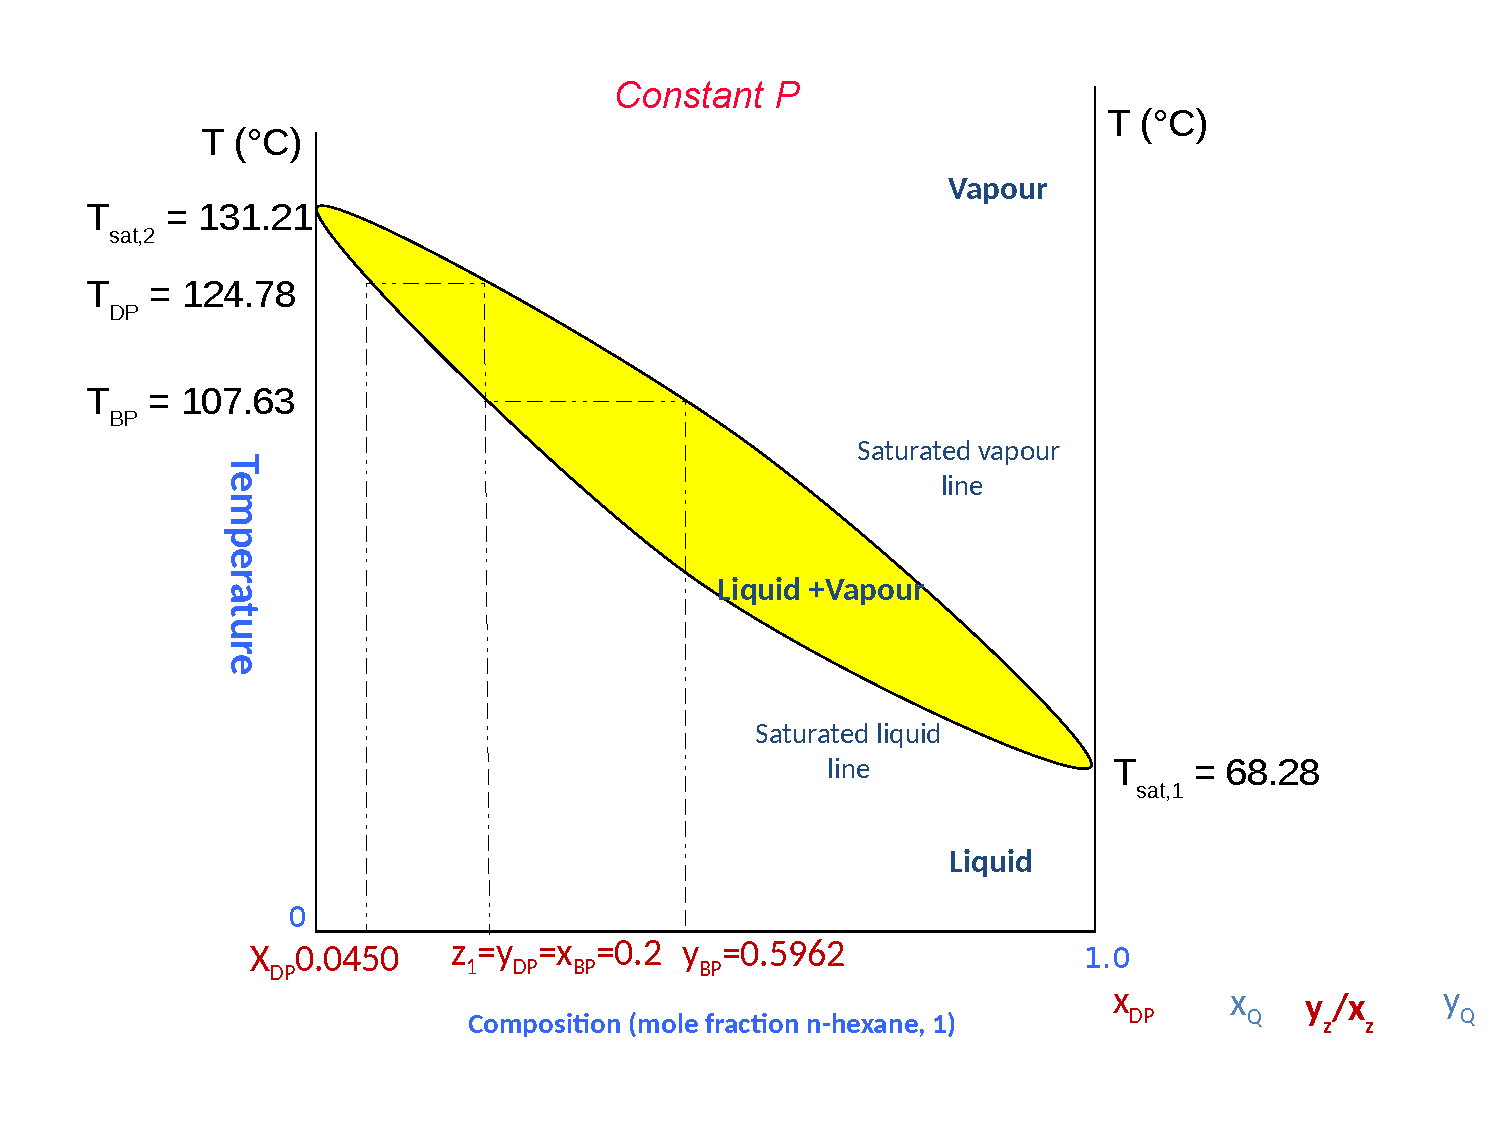
\includegraphics[width=.8\linewidth,clip]{./Pics/VLE_Txy_Diagram}
          \caption{VLE for binary mixture: T-xy diagram at constant pressure.}\label{Figure:Fig1}
        \end{center}
        \end{figure} 
                  }
         \end{enumerate}

         Sauration pressure, $P^{\text{sat}}$, can be obtained from the Antoine equation,
          \begin{displaymath}
            \ln{P^{\text{sat}}} = A - \frc{B}{T+C}
          \end{displaymath}
          where $\left[P^{\text{sat}}\right]$ = kPa and $[T]=[B]=[C] = ^{\circ}$C, with coefficients given in Table~\ref{Practical1:Table2}.
           

\begin{table}[h]
\begin{center}
\begin{tabular}{||c | c c c ||} 
\hline\hline
                           & {\bf A}    &  {\bf B}    & {\bf C}    \\
\hline
{\bf n-hexane}             & 13.8193    & 2696.04     & 224.317    \\  
{\bf n-heptane}            & 13.8622    & 2910.26     & 216.432    \\  
{\bf i-octane}             & 13.6703    & 2896.31     & 220.767    \\ 
{\bf chlorobenze}           & 13.8635    & 3174.78     & 211.700    \\  
\hline\hline
\end{tabular}
\caption{Constants for the Antoine equation for vapour pressure.}
\label{Practical1:Table2}
\end{center}
\end{table}

\end{question}

\clearpage


%%%
%%% Question 02
%%%
\begin{question}
  
%
The methanol steam reforming reaction for hydrogen generation is given by the following chemical reaction,
           \begin{displaymath}
               H_{2}O\text{ (g)} + CH_{3}OH\text{ (g)}  \Leftrightarrow CO_{2}\text{ (g)} + 3H_{2}\text{ (g)},
           \end{displaymath}
with the thermodynamic data at 25$^{\circ}$C,
          \begin{center}
             \begin{tabular}{ c | c c c c }
              \hline
                            &  $H_{2}O\text{ (g)}$ & $CH_{3}OH\text{ (g)}$ & $CO_{2}\text{ (g)}$  & $H_{2}\text{ (g)}$ \\
              \hline
                 $\Delta G^{\circ}_{f,298}$ $\left(\text{kJ mol}^{-1}\right)$ & -228.57 & -161.96 & -394.36 & 0.0 \\
                 $\Delta H^{\circ}_{f,298}$ $\left(\text{kJ mol}^{-1}\right)$ & -241.82 & -200.66 & -393.51 & 0.0 \\
             \end{tabular}
          \end{center}
          where $G^{\circ}_{f,298}$ and $H^{\circ}_{f,298}$ are the standard molar free Gibbs energy and enthalpy of formation, respectively. Determine:

\begin{enumerate}[(a)]
%
   \item The equilibrium constant, $K_{\text{eq}}$, at 25$^{\circ}$C.~\marks{7}
%======================
         \solution{ The equilibrium constant at 25$^{\circ}$C is given by
          \begin{displaymath}
              K_{\text{eq},298} = \exp{\left[-\frc{\Delta G^{\circ}_{\text{mix},298}}{R T}\right]}.
          \end{displaymath}
          The first step is to calculate the standard free Gibbs energy change of the mixture, $\Delta G^{\circ}_{\text{mix},298}$,\solmarks{3/7}
          \begin{eqnarray}
             \Delta G^{\circ}_{\text{mix},298} &=& \left(\Delta G^{\circ}_{f, 298}\right)_{CO_{2}} + 3\left(\Delta G^{\circ}_{f, 298}\right)_{H_{2}} - \left(\Delta G^{\circ}_{f, 298}\right)_{H_{2}O} - \left(\Delta G^{\circ}_{f, 298}\right)_{CH_{3}OH} \nonumber \\
                                                         &=& -3.83 \text{kJ.mol}^{-1} \nonumber
          \end{eqnarray}
          The equilibrium constant can then be calculated,~\solmarks{4/7}
          \begin{displaymath} 
              K_{\text{eq},298} = \exp{\left[-\frc{\Delta G^{\circ}_{\text{mix},298}}{R T} \right]} = \exp{\left[-\frc{3830}{8.314 \times 298.15 } \right]}=4.6884
          \end{displaymath}
}
      
%
   \item The equilibrium constant, $K_{\text{eq}}$, at 60$^{\circ}$C.~\marks{13}
%======================
         \solution{ The equilibrium constant of the chemical reaction can be expressed as a function of the temperature through the Van't Hoff relation: 
          \begin{displaymath}
               \frc{\d}{\d T} \ln{K_{\text{eq}}} = \frc{\Delta H^{\circ}_{\text{mix},298}}{RT^{2}},
          \end{displaymath}
          As data is available at 25$^{\circ}$C (= 298.15 K) and we need it at 60$^{\circ}$C, we can integrate the Van't Hoff equation assuming constant $\Delta H^{\circ}_{298}$,~\solmarks{5/13}
          \begin{eqnarray}
             \Delta H^{\circ}_{\text{mix},298} = \Delta H^{\circ}_{f, 298} &=& \sum \nu_{i}\left(\Delta H^{\circ}_{f, 298}\right)_{i} \nonumber \\
                                                         &=& \left(\Delta H^{\circ}_{f, 298}\right)_{CO_{2}} + 3\left(\Delta H^{\circ}_{f, 298}\right)_{H_{2}} - \left(\Delta H^{\circ}_{f, 298}\right)_{H_{2}O} - \left(\Delta H^{\circ}_{f, 298}\right)_{CH_{3}OH} \nonumber \\
                                                         &=& 48.97 \text{kJ.mol}^{-1} \nonumber
          \end{eqnarray}
          The equilibrium constant at 25$^{\circ}$C is given by
          \begin{displaymath} 
              K_{\text{eq},298} = \exp{\left[-\frc{\Delta G^{\circ}_{\text{mix},298}}{R T} \right]},
          \end{displaymath}
          therefore, we first need to obtain $\Delta G^{\circ}_{\text{mix},298}$, %solmarks{2/13}
          \begin{eqnarray}
             \Delta G^{\circ}_{\text{mix},298} &=& \left(\Delta G^{\circ}_{f, 298}\right)_{CO_{2}} + 3\left(\Delta G^{\circ}_{f, 298}\right)_{H_{2}} - \left(\Delta G^{\circ}_{f, 298}\right)_{H_{2}O} - \left(\Delta G^{\circ}_{f, 298}\right)_{CH_{3}OH} \nonumber \\
                                                         &=& -3.83 \text{kJ.mol}^{-1} \nonumber
          \end{eqnarray}
          Thus,%\solmarks{2/13}
          \begin{displaymath} 
              K_{\text{eq},298} = \exp{\left[-\frc{\Delta G^{\circ}_{\text{mix},298}}{R T} \right]} = \exp{\left[-\frc{3830}{8.314 \times 298.15 } \right]}=4.6884
          \end{displaymath}
           Now, we can proceed with the integration of the Van't Hoff equation,~\solmarks{8/13}
          \begin{displaymath} 
              \frc{\d}{\d T} \left(\ln{K_{\text{eq}}}\right) = \frc{\Delta H^{\circ}_{\text{mix},298}}{RT^{2}} \Longrightarrow \int\limits_{K_{\text{eq}}^{298.15\text{K}}}^{K_{\text{eq}}^{333.15\text{K}}} \d\left(\ln{K_{\text{eq}}}\right) = \frc{\Delta H^{\circ}_{\text{mix},298}}{R}\int\limits_{298.15\text{K}}^{333.15\text{K}}\frc{1}{T^{2}}\d T
          \end{displaymath}
          \begin{eqnarray}
              \ln{\frc{K_{\text{eq}}^{333.15\text{K}}}{K_{\text{eq}}^{298.15\text{K}}}} &=& -\frc{\Delta H^{\circ}_{\text{mix},298}}{R} \left.\frc{1}{T}\right|_{298.15\text{K}}^{333.15\text{K}} \nonumber \\
             K_{\text{eq}}^{333.15\text{K}} &=&  4.6884 \exp{ \left[-\frc{48970}{8.314}\left(\frc{1}{333.15} - \frc{1}{298.15}\right)\right] } = 37.3580 \nonumber 
           \end{eqnarray}

}
%
\end{enumerate}
        For this problem the equilibrium constant at 25$^{\circ}$C is given by
          \begin{displaymath}
              K_{\text{eq},298} = \exp{\left[-\frc{\Delta G^{\circ}_{\text{mix},298}}{R T}\right]}
          \end{displaymath}
          where $\Delta G^{\circ}_{\text{mix},298}$ is the standard free Gibbs energy change of the mixture. Also the Van't Hoff equation is
          \begin{displaymath}
               \frc{\d}{\d T} \ln{K_{\text{eq}}} = \frc{\Delta H^{\circ}_{\text{mix},298}}{RT^{2}},
          \end{displaymath}
          where $\Delta H^{\circ}_{\text{mix},298}$ is the standard enthalpy change of the mixture and $R\left[=\text{8.314 J.}\left(\text{mol.K}\right)^{-1}\right]$ is the molar gas constant.
%
\end{question}

\clearpage



%%%
%%% Question 03
%%%
\begin{question}

%
   \begin{enumerate}[(a)]
%
     \item Two litres of an anti-freezing solution is needed for a cooling process. The solution is prepared by mixing 30 mol$\%$ of methanol in water. What are the volumes of pure methanol and water at 25$^{\circ}$C necessary to prepare solution? Partial molar volumes $\left(\overline{V}\right)$ for methanol and water in a 30 mol$\%$ of methanol solution and their pure species molar volumes $\left(V\right)$, both at 25$^{\circ}$C are:~\marks{8}
       \begin{center}
          \begin{tabular}{ l l l }
                             & $\overline{V}_{i} \left(\text{cm}^{3}.\text{mol}^{-1}\right)$ & $V_{i} \left(\text{cm}^{3}.\text{mol}^{-1}\right)$ \\
               Methanol (1)  & 38.6320                                                     & 40.7270  \\
               Water (2)     & 17.7650                                                     & 18.0680 
          \end{tabular}
       \end{center}
%======================
         \solution{ The molar volume of the 30$\%$-mol of methanol solution is given by,~\solmarks{2/8}
                  \begin{eqnarray}
                     V &=& \frc{V^{T}}{n_{T}} = \frc{\sum\limits_{i=1}^{2}n_{i}\overline{V}_{i}}{n_{T}} = \sum\limits_{i=1}^{2}x_{i}\overline{V}_{i} = x_{1}\overline{V}_{1} + x_{2}\overline{V}_{2} \nonumber \\
                       &=& (0.3)(38.6320) + (0.7)(17.7650) = 24.0251 \text{ cm}^{3}.\text{mol}^{-1} \nonumber
                  \end{eqnarray}
             The total number of moles are:~\solmarks{2/8}
                  \begin{displaymath}
                      n_{T} = \frc{V^{T}}{V} = \frc{2000}{24.0251} = 83.2463 \text{ mol}
                  \end{displaymath}
             The volume of pure methanol and water for the solution are:~\solmarks{4/8}
                  \begin{eqnarray}
                       && V^{\text{pure}}_{1}= x_{1}n_{T}V_{1} = 1017.1116\text{ cm}^{3}\nonumber \\
                       && V^{\text{pure}}_{2}= x_{2}n_{T}V_{2} = 1052.8759\text{ cm}^{3}\nonumber 
                  \end{eqnarray}
}
%
      \item In generating expressions from $G^{E}/RT$ from VLE data, a convenient approach is to plot values of $G^{E}/\left(x_{1}x_{2}RT\right)$ {\it vs} $x_{1}$ and fitting results with an appropriate function. Consider if such data were fit by the expression,
   \begin{displaymath}
       \frc{G^{E}}{x_{1}x_{2} R T} = A + B x_{1}^{2}.
   \end{displaymath}
         From the expression $G^{E}/\left(x_{1}x_{2}RT\right)$, provide equations for the activity coefficient, $\ln{\gamma_{i}}$, as a function of $A$, $B$, $x_{1}$ and $x_{2}$, given~\marks{12}
       \begin{displaymath}
               \ln{\gamma_{i}} = \frc{\overline{G}_{i}^{E}}{RT}.
       \end{displaymath} 
%======================
         \solution{ For a binary mixture, the partial molar property, $\overline{M}$ can be defined as,~\solmarks{2/12}
             \begin{displaymath}
                  \overline{M}_{1} = M + x_{2}\frc{\d M}{\d x_{1}} \hspace{2cm} \text{ and } \hspace{2cm} \overline{M}_{2} = M - x_{1}\frc{\d M}{\d x_{1}}
             \end{displaymath}
             thus with $\overline{M}_{i}=\frc{\overline{G}^{E}_{i}}{RT}$,~\solmarks{3/12}
             \begin{displaymath}
                 \ln{\gamma_{1}} = \frc{\overline{G}^{E}_{1}}{RT} = \frc{G^{E}}{RT} + x_{2}\frc{\d \left(G^{E}/RT\right)}{\d x_{1}} \;\text{ and }\; \ln{\gamma_{2}} = \frc{\overline{G}^{E}_{2}}{RT} = \frc{G^{E}}{RT} - x_{1}\frc{\d \left(G^{E}/RT\right)}{\d x_{1}}.
             \end{displaymath}
             Replacing $x_{2}=1-x_{1}$ in $\frc{G^{E}}{R T} = x_{1}x_{2} \left(A + B x_{1}^{2}\right)$ and differentiating $G^{E}/(RT)$ {\it w.r.t.} $x_{1}$,~\solmarks{5/12}
             \begin{displaymath}
                 \frc{\d \left(G^{E}/RT\right)}{\d x_{1}} = \left(1-2x_{1}\right)A + \left(3-4x_{1}\right)Bx_{1}^{2}
             \end{displaymath}
             The activity coefficient $\left(\text{as a function of } A, B, x_{1} \text{ and } x_{2}\right)$ is then given by,~\solmarks{2/12}
             \begin{eqnarray}
                  && \ln{\gamma_{1}} = x_{1}x_{2}\left(A+Bx_{1}^{2}\right) + x_{2}\left[\left(1-2x_{1}\right)A + \left(3-4x_{1}\right)Bx_{1}\right] \nonumber \\
                  && \ln{\gamma_{2}} = x_{1}x_{2}\left(A+Bx_{1}^{2}\right) - x_{1}\left[\left(1-2x_{1}\right)A + \left(3-4x_{1}\right)Bx_{1}\right] \nonumber 
             \end{eqnarray}
             Alternatively, one could also further develop/simplify the equations above considering $x_{2}=1-x_{1}$.
                
}
%
   \end{enumerate}
%
\end{question}

\clearpage


%%%
%%% Question 04
%%%
\begin{question}
  \begin{enumerate}[a)]
    
%
\item Derive the Maxwell relations below from the fundamental thermodynamic equations.~\marks{11}
\begin{eqnarray}
 \left(\frac{\partial T}{\partial V}\right)_{S} = -\left(\frc{\partial P}{\partial S}\right)_{V}; && 
 \left(\frc{\partial T}{\partial P}\right)_{S} = \left(\frac{\partial V}{\partial S}\right)_{P}; \nonumber \\
 \left(\frc{\partial P}{\partial T}\right)_{V} = \left(\frac{\partial S}{\partial V}\right)_{T}; &&%
  \left(\frac{\partial V}{\partial T}\right)_{P} = -\left(\frc{\partial S}{\partial P}\right)_{T} \nonumber 
\end{eqnarray}
%==========================
%
\solution{First, let's assume a functional $f=f\left(a,b\right)$ and rewrite it as a function of the variables $a$ and $b$,~\solmarks{1/11}
\begin{displaymath}
df = \left(\frc{\partial f}{\partial a}\right)_{b}da + \left(\frc{\partial f}{\partial b}\right)_{a}db
\end{displaymath}
If we define $M=\left(\frc{\partial f}{\partial a}\right)_{b}$ and $N=\left(\frc{\partial f}{\partial b}\right)_{a}$, the equation above becomes~\solmarks{1/11}
\begin{equation}
{\bf df = M da + N db}\label{eqn1}
\end{equation}
Now, if we differentiate $M$ and $N$ with respect to $b$ and $a$, respectively,~\solmarks{1/11}
\begin{displaymath}
\left(\frc{\partial M}{\partial b}\right)_{a} = \frc{\partial^{2} f}{\partial a\partial b}\;\;\text{ and }\;\;\left(\frc{\partial N}{\partial a}\right)_{b} = \frc{\partial^{2} f}{\partial b\partial a}
\end{displaymath}
If the functional $f$ is continuous and differentiable over all domain,~\solmarks{1/11}
\begin{equation}\label{eqn2}
\frc{\partial^{2} f}{\partial a\partial b} = \frc{\partial^{2} f}{\partial b\partial a} \Longrightarrow {\bf \left(\frc{\partial M}{\partial b}\right)_{a} = \left(\frc{\partial N}{\partial a}\right)_{b} }
\end{equation}
The fundamental thermodynamic relations,~\solmarks{1/11} 
\begin{eqnarray}
&& dU = - PdV + TdS \nonumber \\ 
&& dH =   TdS + VdP \nonumber \\
&& dA = - PdV - SdT \nonumber \\
&& dG = - VdP - SdT \nonumber
\end{eqnarray}
have similar shape as Eqn.~\ref{eqn1}, where, for example, in the first relation: ~\solmarks{1/11} 
   \begin{displaymath}
     U = f,\; M=-P,\; N=T,\; \d V=\d a\;\text{ and }\; \d S=\d b. 
   \end{displaymath}
Using relation~\ref{eqn2},~\solmarks{2/11}
   \begin{displaymath}
         -\left(\frc{\partial P}{\partial S}\right)_{V}=\left(\frc{\partial T}{\partial V}\right)_{S}.
   \end{displaymath}
Applying the same to the remaining relations we obtain:~\solmarks{3/11}
\begin{displaymath}
 \left(\frc{\partial T}{\partial P}\right)_{S} = \left(\frac{\partial V}{\partial S}\right)_{P},\; \left(\frc{\partial P}{\partial T}\right)_{V} = \left(\frac{\partial S}{\partial V}\right)_{T}, \text{ and }\; \left(\frac{\partial V}{\partial T}\right)_{P} = -\left(\frc{\partial S}{\partial P}\right)_{T} 
\end{displaymath}
}
%
\item Using the Maxwell relations above, evaluate $\left(\frc{\partial S}{\partial V}\right)_{T}$ for water vapour at 240$^{\circ}$C and molar volume of 0.0258 m$^{3}$.mol$^{-1}$ through the Redlich-Kwong equation of state,
\begin{displaymath}
P = \frc{RT}{V-b} - \frc{a}{V\left(V+b\right)T^{1/2}}
\end{displaymath}
with 
$R$ = 8.314$\times$ 10$^{-5}\;\text{bar.m}^{3}.\left(\text{mol.K}\right)^{-1}$, $a$ = 142.59 $\times$ 10$^{-6}\;\text{bar.m}^{6}.\left(\text{mol.K}\right)^{-2}$ and $b$ = 0.0211 $\times$ 10$^{-3}\text{m}^{3}.\text{mol}^{-1}$.~\marks{9}


%\frc{\text{bar.m}^{3}}{\text{mol.K}}$, $a$ = 142.59 $\times$ 10$^{-6}\; \frc{\text{bar.m}^{6}}{\left(\text{mol.K}\right)^{2}}$ and $b$ = 0.0211 $\times$ 10$^{-3}\frc{\text{m}^{3}}{\text{mol}}$.~\marks{9}
%==========================
\solution{The Maxwell relation ~\solmarks{2/9}
   \begin{displaymath}
      \left(\frc{\partial P}{\partial T}\right)_{V} = \left(\frc{\partial S}{\partial V}\right)_{T}
   \end{displaymath}
    allows to determine $\left(\frc{\partial S}{\partial V}\right)_{T}$ from the PVT relationship in the RK EOS. Thus,~\solmarks{4/9}
\begin{displaymath}
{\bf \left(\frc{\partial P}{\partial T}\right)_{V} = \frc{R}{V-b} + \frc{a}{2 V\left( V + b \right)T^{\frac{3}{2}}}}
\end{displaymath}
Now substituting the variables by their values~\solmarks{3/9}
\begin{displaymath}
  \left(\frc{\partial P}{\partial T}\right)_{V} = \left(\frc{\partial S}{\partial V}\right)_{T} = 3.2342\times 10^{-3} \text{bar.K}^{-1} = 3.2342\times 10^{-1}\frc{\text{kJ}}{\text{m}^{3}.\text{K}}
\end{displaymath}

}
  \end{enumerate}
\end{question}

\clearpage

%%%
%%% QUESTION 05
%%%
\begin{question}
   Scientists in China are investigating the feasibility of a novel enhanced geothermal system (EGS) technology to produce power and heat in the Gonghe basin in the northwestern province of Qinghai. Their initial well test demonstrated that at a depth of 3705 meters, the geological formation temperature is of 235$^{\circ}$C.  They predicted that 5.6805 kg.s$^{-1}$ of brine $\left(m_{\text{br}}\right)$ can be extracted from the reservoir and, at the top of the well, pressure and temperature of the fluid are 15 bar and 200$^{\circ}$C, respectively. In their preliminary plant design (Fig.~\ref{Figure:Fig1}), 2 turbines would produce 3.5 MW of power, whilst a condenser (fed with cold water, A) would extract 15.75 MW of heat from the brine before re-injection into the geothermal reservoir. 
      \begin{figure}[h]
        \begin{center}
          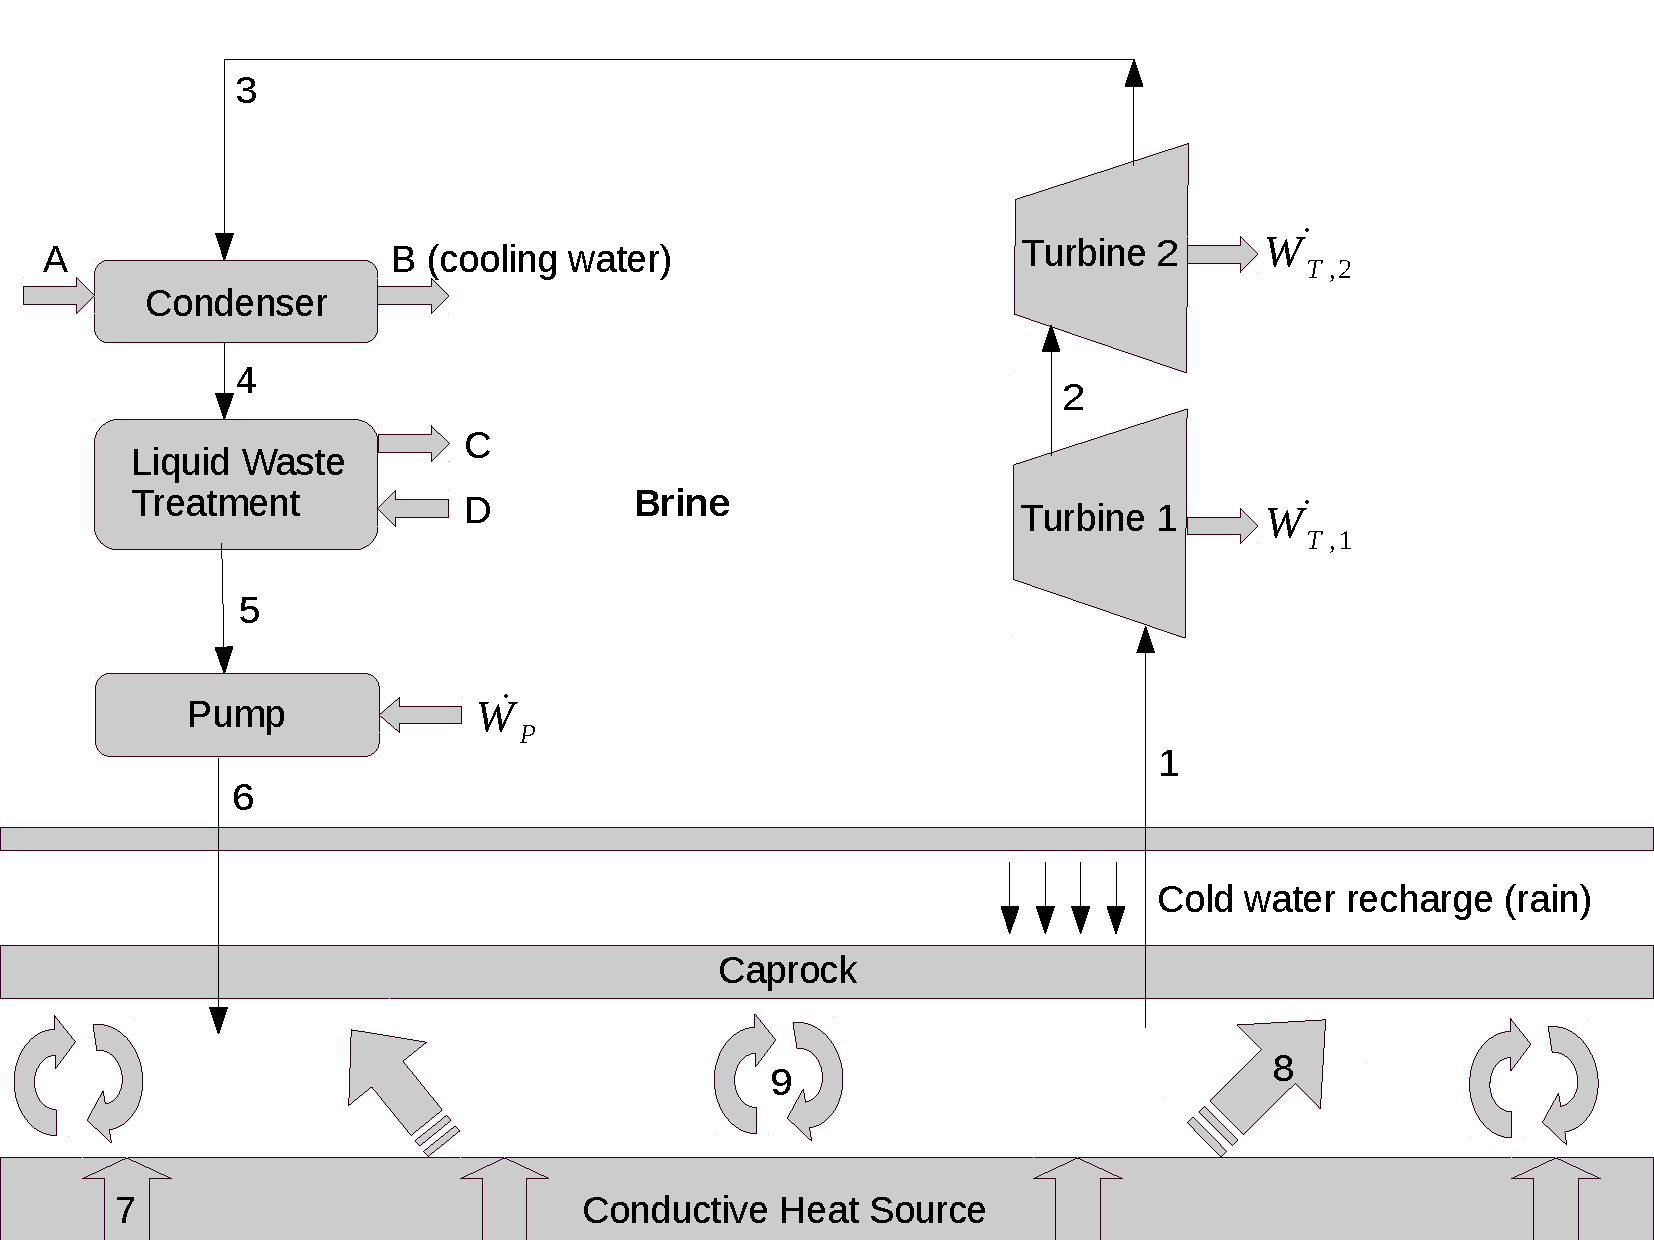
\includegraphics[width=.8\linewidth,clip]{./Pics/Exam2_PowerPorousMedia.pdf}
          \caption{Schematics of geothermal source exploration for power and heat production.}\label{Figure:Fig1}
        \end{center}
      \end{figure}
      
      \begin{table}[h]
        \begin{center}
          \begin{tabular}{||c|c|c|c|c|c||}
            \hline\hline
                {\bf Stream} & {\bf Pressure} & {\bf Temperature} & {\bf Fluid} & {\bf Specific enthalpy} & {\bf Specific entropy} \\
                             & {\bf (bar)}    & {\bf $\left(^{\circ}\text{C}\right)$}& &  {\bf $\left(\text{kJ.kg}^{-1}\right)$} & {\bf $\left(\text{kJ.kg}^{-1}\text{.K}^{-1}\right)$} \\  
            \hline\hline
                {\bf 1}      &   15           &   200              & (i)        &  (ii)                   &   (iii)                  \\
            \hline
                {\bf 2}      &   7            &   180              & dry vapour &   (iv)                  &   (v)                     \\ 
            \hline
                {\bf 3}      &   5            &   --               & (vi)       &   (vii)                 &    (viii)                 \\
            \hline
                {\bf 4}      &   --           &   (ix)             & --        &    (x)                   &    --                     \\
            \hline
                {\bf 5}      &   4.50         &   147.90           & --        &    (xi)                  &    --                     \\
            \hline
                {\bf 6}      &   25.00        &   --               & (xii)      &    (xiii)               &    --                     \\
            \hline
                {\bf A}      &   --           &   20               & Cold water  &   --                   &    --                     \\
            \hline
                {\bf B}      &   --           &   --               & Hot water  &   --                   &    --                     \\
            \hline
                {\bf C}      &   --           &   --               & Liquid residue&   --                   &    --                     \\
            \hline
                {\bf D}      &   --           &   --               & Cold water  &   --                   &    --                     \\
            \hline\hline
          \end{tabular}
           \caption{Thermal-physical​ conditions​ ​of​ all​ streams​ ​from​ ​Fig.​~\ref{Figure:Fig1}}\label{Table:Tab1}
        \end{center}
      \end{table}

       Before re-injection, contaminants are removed from the brine stream at a rate of 0.1 kg.s​$^{-1}$ (stream C) and, in order to replenish the geothermal reservoir, 10 kg.s​$^{-1}$ of cold water is added into the brine stream (D). Your task is to check if the predicted power and heat production are correct, therefore: 
  \begin{enumerate}[a)]
     \item Calculate conditions (i-xiii) from Table~\ref{Table:Tab1};~\marks{13}
         \solution{Following the streams:
            \begin{enumerate}[1)]
               \item At $P_{1}=15$ bar and $T_{1}=200^{\circ}$C, brine is at {\it superheated vapour} state {\bf (i)}\solmarks{1/13} with $h_{1}=2796.8\text{ kJ.kg}^{-1}$ {\bf (ii)}\solmarks{1/13} and $s_{1}=6.4546\text{ kJ.kg}^{-1}$ {\bf (iii)}\solmarks{1/13};
               \item At $P_{2}=7$ bar, brine is a dry vapour with $h_{2}=2763.5\text{ kJ.kg}^{-1}$ {\bf (iv)}\solmarks{1/13} and $s_{2}=6.7080\text{ kJ.kg}^{-1}$ {\bf (v)}\solmarks{1/13};
               \item At $P_{3}=5$ bar, an isentropic expansion of the fluid occurs in Turbine 2, \ie $s_{3}=s_{2}=6.7080\text{ kJ.kg}^{-1}$ {\bf (viii)}\solmarks{1/13}. At such pressure, the saturation table gives:
                 \begin{displaymath}
                   \begin{cases}
                      h_{f} = 640.23\text{ kJ.kg}^{-1}, & s_{f} = 1.8607\text{ kJ.(kg.K)}^{-1}, \\
                      h_{g} = 2748.7\text{ kJ.kg}^{-1}, & s_{g} = 6.8212\text{ kJ.(kg.K)}^{-1}.
                   \end{cases}
                 \end{displaymath}
                 As $s_{3}<s_{g}$, the fluid is {\it wet vapour} {\bf (vi)}~\solmarks{1/13}. In order to calculate the enthalpy of this stream, we first need​​ to obtain the quality​ of the vapour through,\solmarks{1/13}
                 \begin{displaymath}
                   \begin{cases}
                     x_{3} = \frc{s_{3}-s_{f}}{s_{g}-s_{f}} = 0.9772, & \\
                     x_{3} = \frc{h_{3}-h_{f}}{h_{g}-h_{f}} & \Longrightarrow h_{3} = 2700.626 \text{ kJ.kg}^{-1}\textbf{ (vii)}
                   \end{cases}
                 \end{displaymath}
               \item The condenser removes heat from the brine stream with no pressure drop, therefore $P_{4}=P_{3}=5$ bar with $T_{4}=T_{\text{sat}}=151.9^{\circ}$C {\bf (ix)}~\solmarks{1/13}. Fluid leaving the condenser is saturated liquid with $h_{4}=h_{f}=640.23\text{ kJ.kg}^{-1}$ {\bf (x)}\solmarks{1/13};
               \item After the liquid waste treatment unit, the brine stream is at $P_{5}=4.5$ bar and the saturated temperature is $T_{\text{sat}}=T_{5}=147.9^{\circ}$C, thus the brine is at saturated liquid state with $h_{5}=623.25\text{ kJ.kg}^{-1}$ {\bf (xi)}\solmarks{1/13} and $v_{5}=1.0882\times 10^{-3}\text{ m}^{3}\text{.kg}^{-1}$;
               \item At the pump, $P_{6}=25$ bar, the fluid undertakes an isentropic compression and from the fundamental thermodynamic relation:
                   \begin{displaymath}
                      Tds = dh - vdP.
                   \end{displaymath}
                   However, as $ds = 0$ (\ie isentropic) and, assuming that the fluid is incompressible, \ie $v_{6}=v_{5}$,~\solmarks{1/13}
                   \begin{displaymath}
                      \int dh = \int vdP \;\;\Longrightarrow h_{6}=h_{5} + v_{5}\left(P_{6}-P_{5}\right) = 625.4808\text{ kJ.kg}^{-1} \text{\bf  (xiii)}.
                   \end{displaymath}
                    At 25 bar, the saturated liquid enthalpy, $h_{f}$, is 962.11 kJ.kg$^{-1} > h_{6}$, therefore the brine is at {\it subcooled liquid state} {\bf (xii)}. ~\solmarks{1/13}
            \end{enumerate}
         }
%%%%%%%%%%%%%%%%%%%%%%       
       \item Are the predictions of power and heat correct? If not, calculate the power produced by the Turbines and heat extracted by the Condenser;~\marks{3}
         \solution{ Total power produced by the turbines are~\solmarks{1/3}
           \begin{eqnarray}
              \dot{W}_{T} &=& \dot{W}_{T,1} + \dot{W}_{T,2} =  \dot{m}_{br}\left(h_{2}-h_{1}\right) + \dot{m}_{br}\left(h_{2}-h_{1}\right) \nonumber \\
                         &=& -546.30\text{kJ.kg}^{-1} =  0.5463\text{ MW} \nonumber
           \end{eqnarray}
           The heat extracted by the condenser is~\solmarks{1/3}
              \begin{displaymath}
                  \dot{Q}_{c} = \dot{m}_{br}\left(h_{4}-h_{3}\right) = -11704.4771\text{ kJ.kg}^{-1} = 11.7045\text{ MW}
              \end{displaymath}
              Thus, scientists over-predicted power production and heat extraction from the power plant~\solmarks{1/3}.
           }
     \item Sketch the temperature $\times$ specific entropy $\left(Ts\right)$ diagram of the process involving streams (1)-(4), indicating:~\marks{4}
       \begin{itemize}
          \item entropies and temperatures;
          \item liquid saturated line;
          \item vapour saturated line;
          \item critical point;
          \item isobars.
       \end{itemize}
       \solution{
         Marks:
         \begin{itemize}
            \item entropies and temperatures;\solmarks{2/4}
          \item liquid and vapour saturated line;\solmarks{1/4}
          \item isobras and critical point.\solmarks{1/4}
         \end{itemize}
         
        \begin{center}
          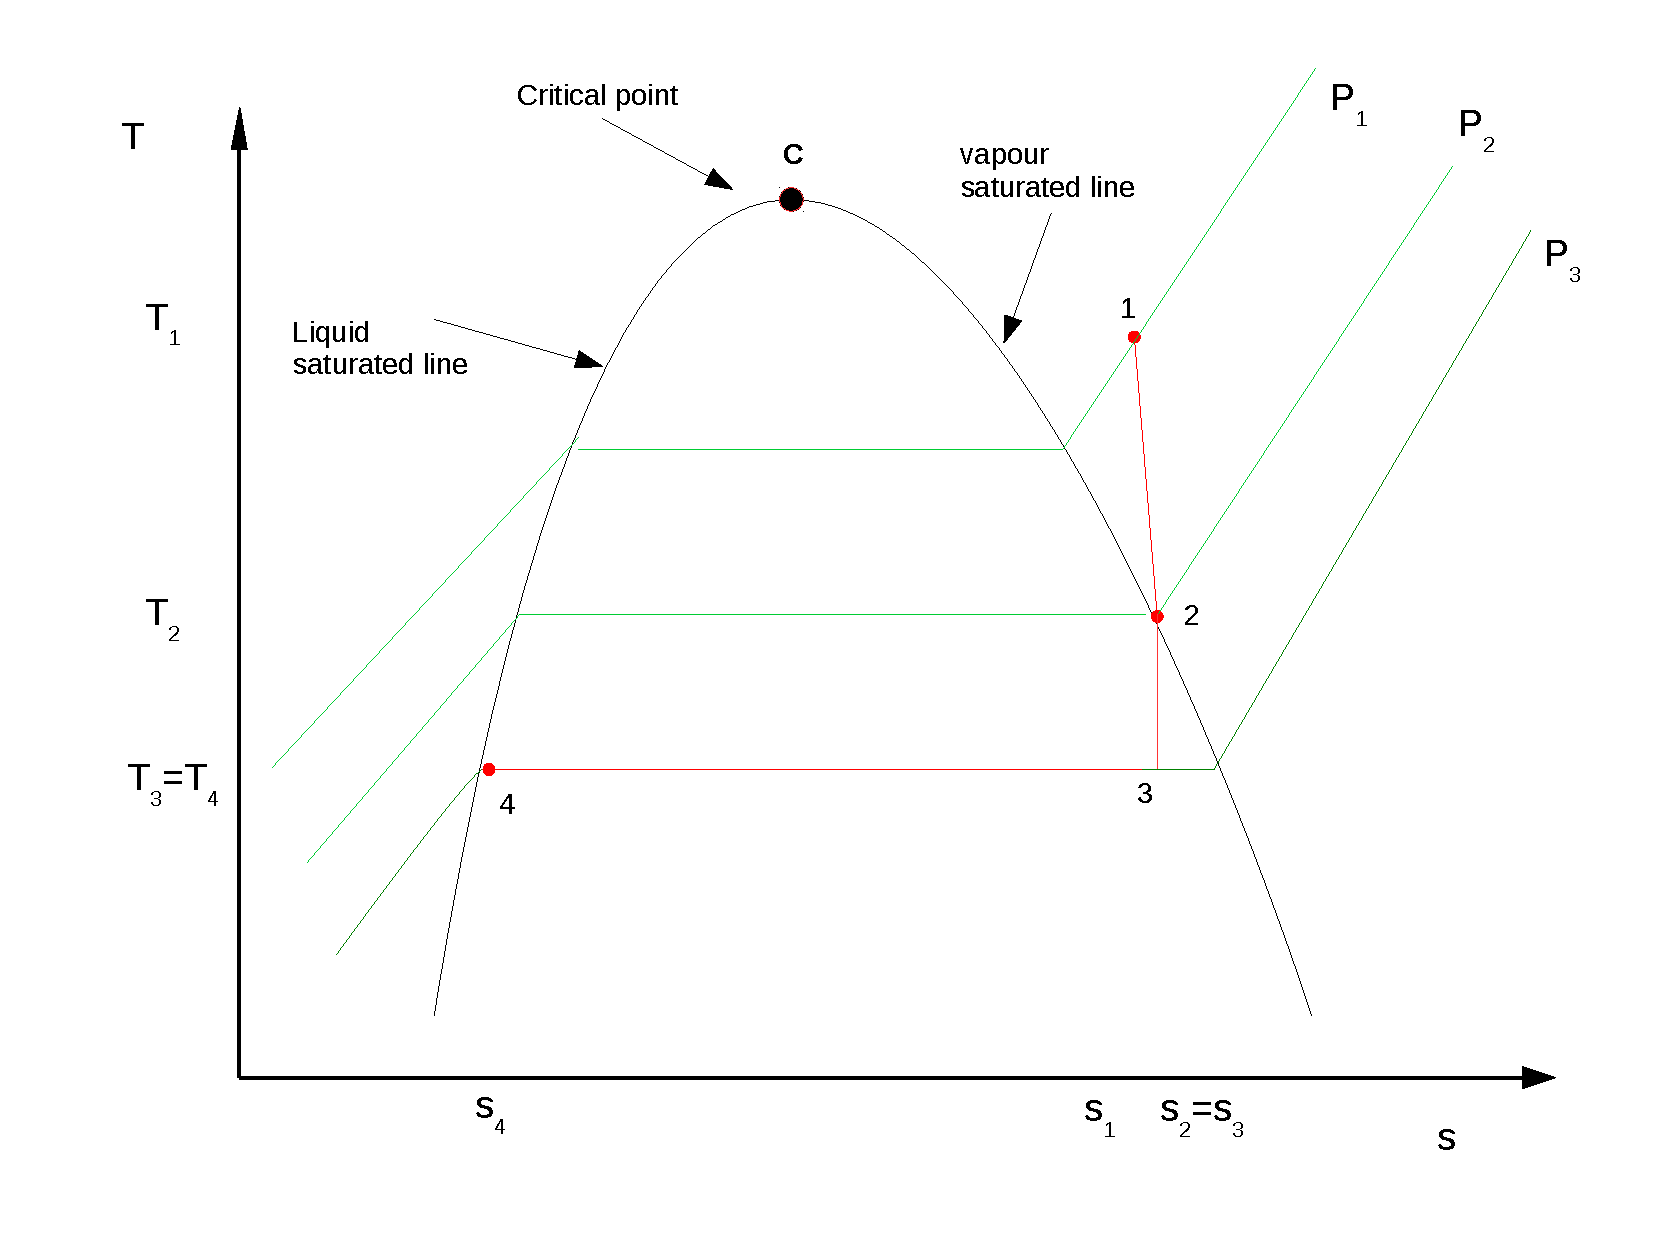
\includegraphics[width=.8\linewidth,clip]{./Pics/Exam_TSDiagram}
        \end{center}
        }
  \end{enumerate}
  In order to solve this problem, assume that brine has the same thermodynamic properties as water. Also, assume that ideal isentropic expansion and compression occurs at Turbine 2 and the Pump, respectively. Finally, assume that liquid brine behaves as an incompressible fluid.
\end{question}

\clearpage

\vfill
\paperend
 


\vfill 



\begin{comment}
{
  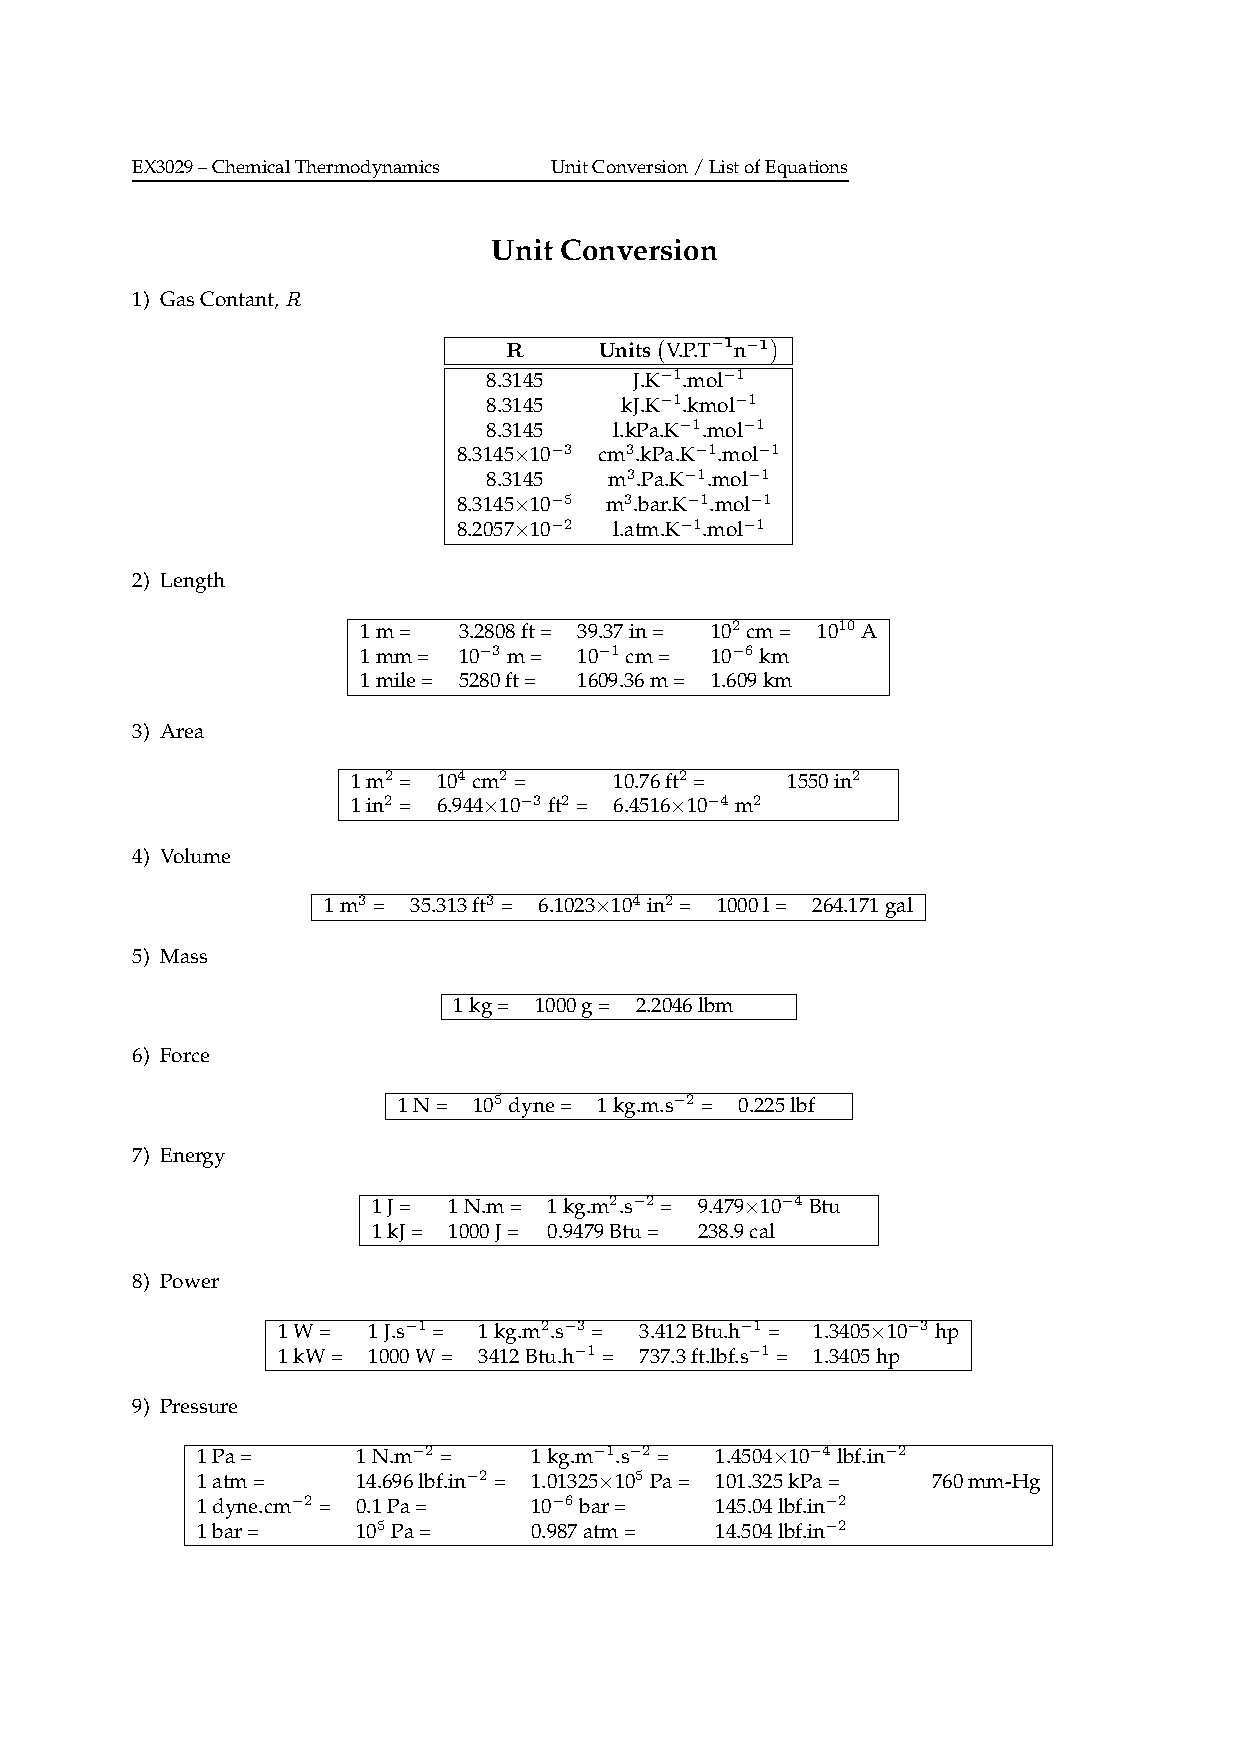
\includepdf[pages=-,fitpaper]{./Pics/EquationsList}
  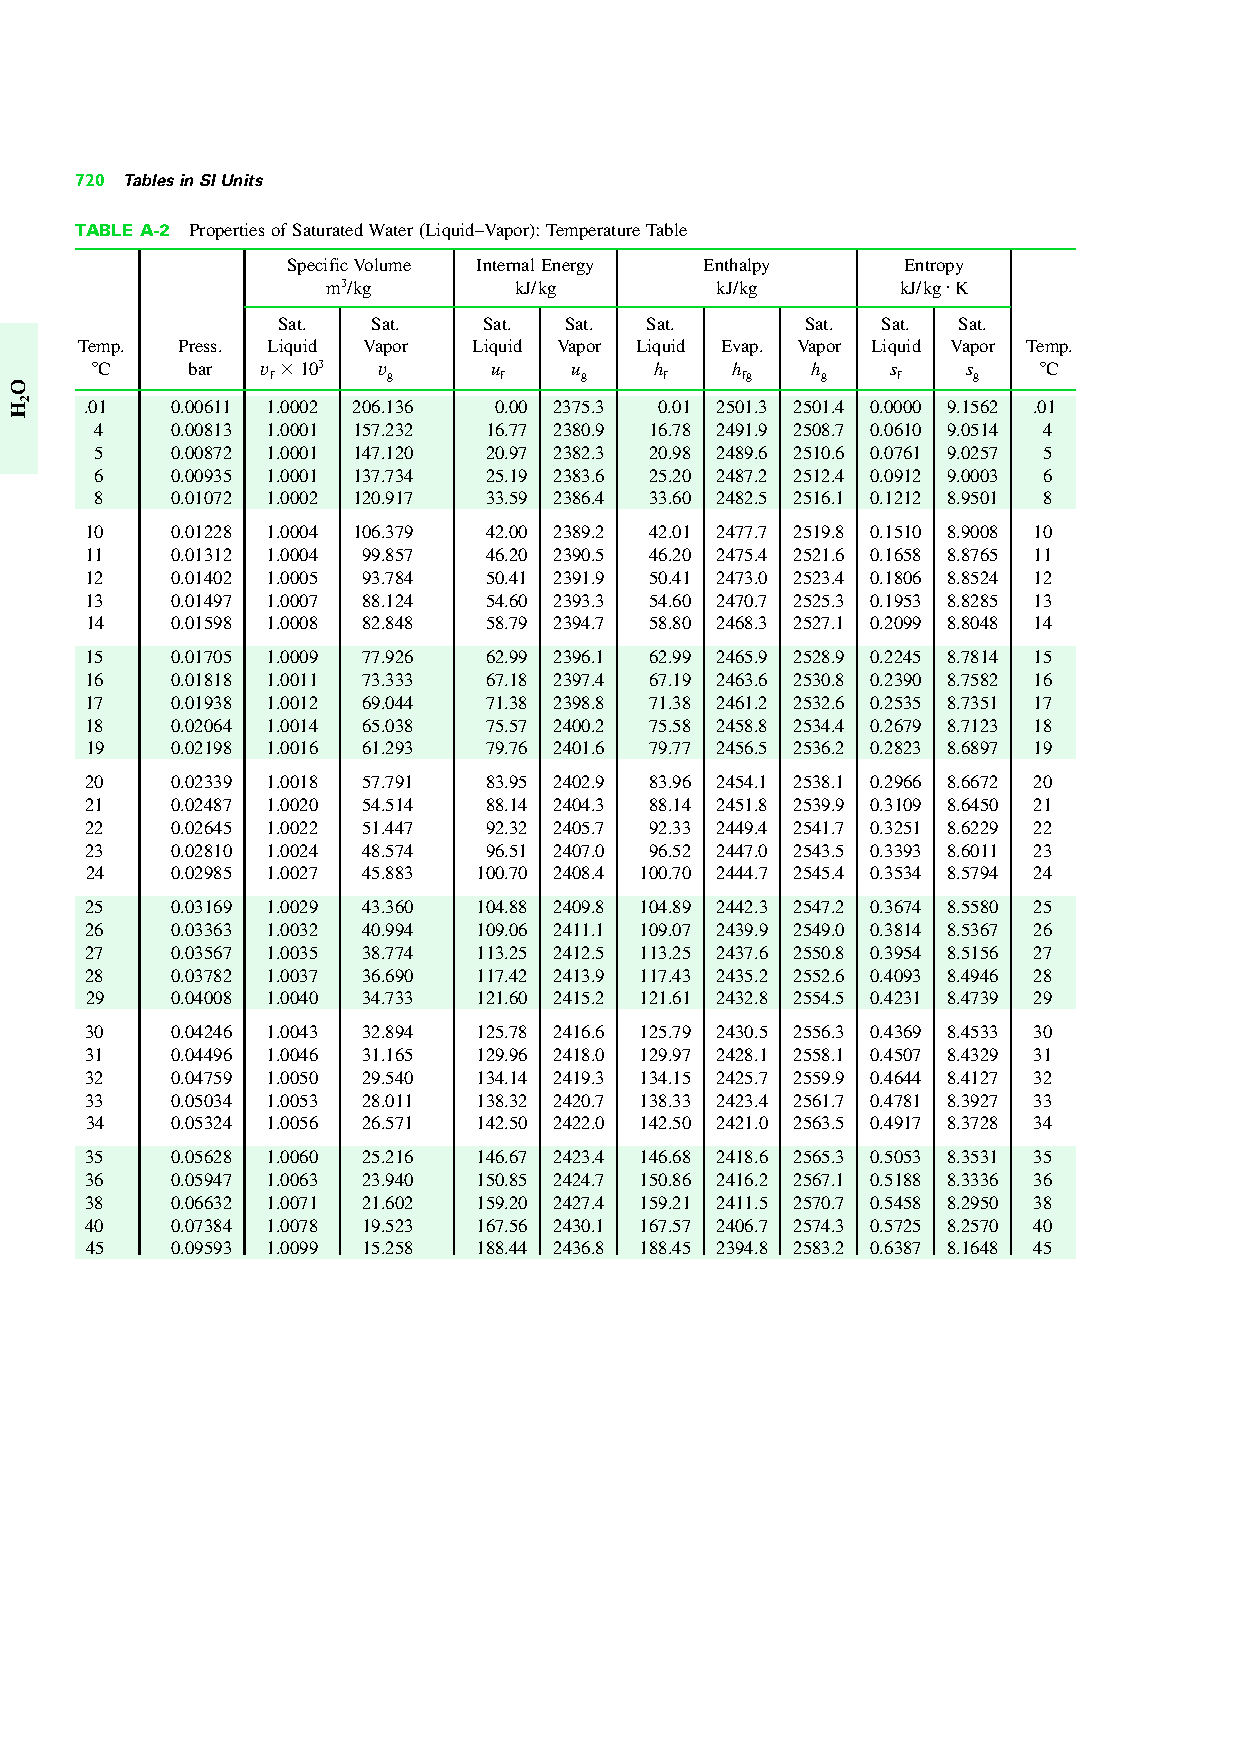
\includepdf[pages=-,fitpaper]{./Appendix4Exams/Tables/SatProp_H2O}
}
\end{comment}



\end{document}
